\chapter{Parallel Computing 2D Voronoi Diagrams Using Untransformed Sweepcircles}

This chapter presents a new algorithm, called {\em
untransformed sweepcircle}, for constructing Voronoi diagram in
$\mathbb{R}^2$. Starting with a degenerate circle (of zero radius)
centered at an arbitrary location, as the name suggests, our
algorithm sweeps the circle by increasing its radius across the
plane. At any time during the sweeping process, each site inside the
sweep circle defines an ellipse composing of points equidistant from
that point and from the sweep circle. The union of all ellipses
forms the beach curve, a star shape inside the sweep circle which
divides the portion of the plane within which the Voronoi diagram
can be completely determined, regardless of what other points might
be outside of the sweep circle. As the sweep circle progresses, the
intersection of expanding ellipses defines the Voronoi edges. We
show that the sweep line algorithm is the degenerate form of the
proposed sweep circle algorithm when the circle center is at
infinity, and our algorithm has the same time and space complexity
as the sweep line algorithm. Our untransformed sweepcircle algorithm
is flexible in allowing multiple circles at arbitrary locations to
sweep the domain simultaneously. The parallelized implementation is
pretty easy without complicated numerical computation; the most
complicated case is nothing but an arc-cosine operation.
Furthermore, our algorithm supports the additively weighted Voronoi
diagrams of which the Voronoi edges are hyperbolic and straight line
segments. We demonstrate the efficacy of our parallel sweep circle
algorithm using GPU.


The rest of the chapter is structured as follows.Section~\ref{sec:sweepcircle-preliminaries} briefly reviews some math prelimitaries.
Then we introduce the key concepts and properties of the untransformed sweepcircle algorithm in
Section~\ref{sec:sweepcircle-algorithm} and then present the parallel implementation on modern GPUs in Section~\ref{sec:sweepcircle-parallel}.
We provide the detailed experimental results in Section~\ref{sec:sweepcircle-results} and discuss the fundamental differences between
the untransformed sweepcircle algorithm and Dehne~\& Klein's sweepcircle method~\cite{Dehne_Klein:1987} in Section~\ref{sec:sweepcircle-discussion}.
Finally in Section~\ref{sec:sweepcircle-summary}, we conclude the chapter and suggest several future research directions.

\section{Preliminaries}\label{sec:sweepcircle-preliminaries}
\vspace{-0.1in} This section briefly reviews the theoretical
background of Voronoi diagram and Fortune's sweep line algorithm.

Let $S=\{s_1,s_2,\cdots,s_n\}$ be a set of points (called {\em sites}) in
$\mathbb{R}^d$. The Voronoi cell $Vor(s_i)$ of a site $s_i$ is
\[
Vor(s_i)=\{x\in\mathbb{R}^d|\|x-s_i\|\leq\|x-s_j\|~\forall j, j\neq
i\},
\]
where $\|p-q\|$ denotes the Euclidean distance between points $p$
and $q$. The Voronoi cell $Vor(s_i)$ is the set of all the points
$x$ that are at least as close to $s_i$ as to any other site $s_j$
in $S$. All the Voronoi cells form a partition of the given space.
It is well known that each Voronoi cell is convex and contains
exactly one site. A Voronoi cell is unbounded if and only if the
corresponding site lies on the convex hull of $S$. The number of
Voronoi edges and vertices is $O(n)$.

The Delaunay triangulation is the dual structure of the Voronoi
diagram. By dual, we mean two Voronoi sites are
connected by a line segment if they share a Voronoi edge.
Figure~\ref{fig:voronoiexample}(a) shows an example of 2D Voronoi
diagram and its dual Delaunay triangulation.

\begin{figure}[htbp]

\centering{
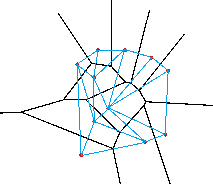
\includegraphics[height=2.4in]{figs/sweepcircle/voronoiexample.png}
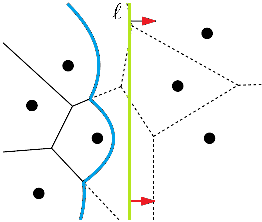
\includegraphics[height=2.4in]{figs/sweepcircle/sweepline2.png}\\
\makebox[1.55in]{(a)}\makebox[1.55in]{(b)}\\
} \vspace{-0.1in}\caption{(a) An example for the Voronoi diagram
(black) and its dual Delaunay triangulation (blue). (b) Fortune's
sweep line algorithm~\cite{Fortune1986} maintains a sweep line
(green) and a beach line (blue) moving from left to right. The
region left to the beach line contains the partial Voronoi diagram
with a correctly computed topological structure (the solid black
lines). The right region corresponds to the to-be-determined part of
the Voronoi diagram. }\label{fig:voronoiexample}
\vspace{-2mm}
\end{figure}

Fortune's sweep line algorithm~\cite{Fortune1986} maintains a sweep
line and a beach line as the algorithm progresses. Without loss of
generality, assume the sweep line is a vertical straight line moving
from left to right across the plane. Each site left of the sweep
line defines a parabola of points equidistant from that point and
from the sweep line. The beach line is the boundary of the union of
these parabolas, which splits the plane into two regions: the left
region contains a partial Voronoi diagram with a correctly computed
topological structure, and the right region corresponds to
to-be-determined part of the Voronoi diagram. As the sweep line
progresses, the vertices of the beach line, at which two parabolas
cross, trace out the edges of the Voronoi diagram, see
Figure~\ref{fig:voronoiexample}(b). Some important properties of the
sweep line algorithm are as follows:
\begin{itemize}
\item The beach line intersects each horizontal line at exactly one point.
\item When a parabolic segment disappears,  a Voronoi vertex is generated.
\item For the region on the left hand side of the beach line, the Voronoi diagram has been determined, while the region on the right corresponds to the to-be-determined Voronoi
diagram.
\item The sites on the left of the beach line can be classified into two
groups: {\em fixed} sites whose Voronoi cell has been totally
determined and {\em active} sites whose Voronoi cell is under
computation.
\item Suppose $x_i$ is an active site, then the parabolic segment determined by $x_i$ is totally inside $x_i$'s Voronoi cell.
\end{itemize}


In the sweep line algorithm, a balanced binary search tree is used to
maintain the combinatorial structure of the beach line, and a
priority queue listing potential pending events that possibly change the
beach line structure. It can be shown that there are $O(n)$ events
to process and $O(\log n)$ time required to process each event, and hence the total
time is $O(n\log n)$.



Although the sweep line algorithm is conceptually elegant and widely
adopted, it is non-trivial to parallelize and implement it on modern
GPUs. As shown in Figure~\ref{fig:sweeplineDrawback}, to compute the
Voronoi diagram for the square domain in parallel, we partition it
to a set of square-shaped blocks with side length $\tau$, and then
run the sweep line algorithm for each block independently. Without
loss of generality, we assume that at least one site is contained in
the green block. It can be shown that only the sites in the red
round-cornered rectangle, $(4\sqrt{2}+2\pi+1)\tau^2$ in size, affect
the Voronoi diagram of the green block. Therefore, we need to place
a sweep line at the left boundary of the red round-cornered
rectangle (see Figure~\ref{fig:sweeplineDrawback}(a)) and consider
the sites located inside this area in the subsequent sweeping
process. In this example, as sites $A$ and $B$ are inside the red
region, the sweep line algorithm results in a Voronoi edge bisecting
$A$ and $B$ (see the yellow line segment in
Figure~\ref{fig:sweeplineDrawback}(b)). However, the correct Voronoi
diagram (the dotted blue lines in
Figure~\ref{fig:sweeplineDrawback}(a)) consists of only part of the
bisecting line of $A$ and $B$ due to the existence of site $C$,
of which is outside of the red region. In fact, it can be shown that
only the Voronoi diagram inside the green region is correct and
contributes to the final result. Therefore, we have to trim the
computed Voronoi diagram (of the entire red region) with the
centered green region to get the final result. In other words, each
sweep line algorithm computes the Voronoi diagram for a region of
size $(4\sqrt{2}+2\pi+1)\tau^2$, but only the result inside the
centered region of size $\tau^2$ is used. Roughly speaking,
$1-\frac{1}{(4\sqrt{2}+2\pi+1)}=92.3\%$ computation is totally
wasted. Due to these drawbacks, it is difficult to parallelize the
sweep line algorithm in an efficient and effective manner. To our
knowledge, there is no such algorithm known to the community.
\begin{figure}[htbp]
\centering
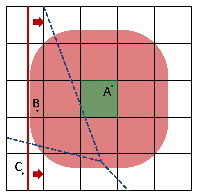
\includegraphics[height=2.45in]{figs/sweepcircle/sweeplineDrawback1.png}
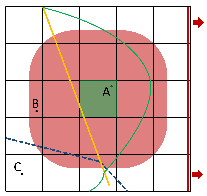
\includegraphics[height=2.45in]{figs/sweepcircle/sweeplineDrawback2.png}\\
\makebox[1.45in]{(a)}\makebox[1.45in]{(b)}\\
\caption{(a) To compute the Voronoi diagram for the
green region, one has to apply the sweep line algorithm to a much
larger domain (in red). (b) At the conclusion of the sweep line
algorithm, one has to trim the computed Voronoi diagram with the
centered region. The doted blue lines are the real Voronoi
edges.}\label{fig:sweeplineDrawback}
\end{figure}

The proposed untransformed sweepcircle algorithm overcomes the drawbacks of the
sweep line algorithm, and can be naturally extended to parallel
setting.

\vspace{-0.1in}
\section{Untransformed Sweepcircle Algorithm}\label{sec:sweepcircle-algorithm}
\vspace{-0.1in}
\subsection{Algorithm Description}
In contrast to the sweep line algorithm which propagates the
sweep/beach line from left to right, our algorithm starts with a
degenerate circle at an arbitrary location and then sweeps the circle
by increasing its radius to cover the entire domain. Our untransformed sweepcircle algorithm contains four fundamental elements:
\begin{itemize}
\item The \textbf{sweep circle}, centered at the user-specified or a random location $c$, sweeps the plane by increasing its radius. The initial radius is usually set to zero.
\item The \textbf{beach curve} is a set of consecutive elliptic segments, each of which bisects a site and the sweep circle. The beach curve splits the
plane into two regions: the inside region contains a partial Voronoi
diagram with a correctly computed topological structure, and the
outside region corresponds to an undetermined part of the Voronoi
diagram that will be computed later.
\item A \textbf{touching event} occurs when the sweep circle touches a new site. As a result, a new elliptic segment is inserted into the current beach curve.
\item A \textbf{vanishing event} occurs when an elliptic segment
disappears. Consequently, a new Voronoi vertex is generated.
\end{itemize}

Figure~\ref{fig:sweepcircleprocess} illustrates the basic idea of
sweep circle for a two-site example. Initially, we place a
degenerate circle (i.e., a point) at the user-specified or at random
location $c$. Assume the circle center does not coincide with any
sites. The circle grows until it touches the closest site, say
$s_1$, which triggers the first touching event (see (b)). As a
result, we construct a degenerate ellipse with focus points $s_1$
and $c$, satisfying $\|x-s_1\|+\|x-c\|=R$, where $R=\|c-s_1\|$ is the
radius of the current sweep circle. Clearly, the initial beach curve
is a line segment (i.e., degenerate ellipse). Throughout the
sweeping process, the ellipse always satisfies the constraint
$\|x-s_1\|+\|x-c\|=R$ for the increasing radius $R$. It can be shown
that the ellipse is the bisector of $s_1$ and the sweep circle
$\odot(c,R)$. Furthermore, the beach curve is always inside the
sweep circle (see (c)). The next event (again, a touching event)
occurs when the sweep circle reaches the second site $s_2$, which
creates an ellipse $\|x-s_2\|+\|x-c\|=R$ (now $R=\|c-s_2\|$. This
newly generated ellipse is inserted into the current beach curve.
Thus, the updated beach curve contains two elliptic segments, each
of which is the bisector of the sweep circle and the corresponding
site (see (d)). As the sweep circle progresses, the vertices of the
beach curve, at which two ellipses cross, trace out the bisector (in
red) of $s_1$ and $s_2$ (see (e)). Note that the \textit{continuous}
animation is used to illustrate the basic concept of sweep circle.
In fact, our algorithm sweeps the circle and processes the events in
a \textit{discrete} manner.

Figure~\ref{fig:sweepcircleExample} shows the circle sweeping on a
domain with five sites. The key idea of our untransformed sweepcircle algorithm
is to maintain the (circular) ordered list of elliptic segments and
trace out the vertices of the beach curve. The two neighboring (in
circular order) elliptic segments correspond to an {\em active}
Voronoi edge and the two neighboring active edges (in circular
order) are joined by an elliptic segment. When an elliptic segment
vanishes (i.e., a vanishing event occurs), the two neighboring
active edges meet at a point, which defines a Voronoi vertex (see
the insets in Figure~\ref{fig:sweepcircleExample}~(d),(f),(g)). When
the sweep circle touches a new site (i.e., a touching event occurs),
a new Voronoi edge is generated. The discrete events are maintained
in a priority queue sorted by the distances of the corresponding
sites to the center $c$ (from near to far). Throughout the
algorithm, the Voronoi diagram inside the beach curve has been
determined. The algorithm stops when the priority queue is empty and
at this moment the complete Voronoi diagram is known. The essential
data structures in the untransformed sweepcircle algorithm include the Voronoi
diagram, the beach curve and the event manager, shown as follows:

\noindent\makebox[6mm]{}{//2D point, vector or interval}\\
\noindent\makebox[6mm]{}{typedef pair$<$double,double$>$ double2;}\vspace{3mm}\\
\noindent\makebox[6mm]{}{//Lists of sites and Voronoi vertices}\\
\noindent\makebox[6mm]{}{vector$<$double2$>$} SiteList;\\
\noindent\makebox[6mm]{}{vector$<$double2$>$} VoronoiVertexList;\vspace{3mm}\\
%\noindent\makebox[6mm]{}{//Voronoi edges}\\
\noindent\makebox[6mm]{}{struct VoronoiEdge} \{\\
\noindent\makebox[6mm]{}\makebox[6mm]{}//two endpoints of the edge\\
\noindent\makebox[6mm]{}\makebox[6mm]{}{int} vert1,~vert2;\\
\noindent\makebox[6mm]{}\makebox[6mm]{}//two sites contributing to the bisector\\
\noindent\makebox[6mm]{}\makebox[6mm]{}{int} site1,~site2;\\
\noindent\makebox[6mm]{}\};\\
\noindent\makebox[6mm]{}{vector$<$VoronoiEdge$>$} VoronoiEdgeList;\vspace{3mm}\\
\noindent\makebox[6mm]{}//An active edge, shared by two consecutive elliptic\\
\noindent\makebox[6mm]{}//segments, contains one fixed endpoint and an\\
\noindent\makebox[6mm]{}//extending direction\\
\noindent\makebox[6mm]{}{struct ActiveEdge} \{\\
\noindent\makebox[6mm]{}\makebox[6mm]{}{int} indexFixedEndpoint; \\
\noindent\makebox[6mm]{}\makebox[6mm]{}{double2 extendingDirection;\\
\noindent\makebox[6mm]{}\makebox[6mm]{}{EllipticSegment*} leftSegment;\\
\noindent\makebox[6mm]{}\makebox[6mm]{}{EllipticSegment*} rightSegment;\\
\noindent\makebox[6mm]{}\};\\
\noindent\makebox[6mm]{}{struct EllipticSegment} \{\\
\noindent\makebox[6mm]{}\makebox[6mm]{}//One focus point is the center of the sweep circle\\
\noindent\makebox[6mm]{}\makebox[6mm]{}{double2 circleCenter;\\
\noindent\makebox[6mm]{}\makebox[6mm]{}//The other focus point is a site\\
\noindent\makebox[6mm]{}\makebox[6mm]{}{int} indexActiveSite;\\
\noindent\makebox[6mm]{}\makebox[6mm]{}//Sandwiched by two neighboring active edges.\\
\noindent\makebox[6mm]{}\makebox[6mm]{}{ActiveEdge*} leftActiveEdge;\\
\noindent\makebox[6mm]{}\makebox[6mm]{}{ActiveEdge*} rightActiveEdge;\\
\noindent\makebox[6mm]{}\};\\
\noindent\makebox[6mm]{}{//The beach curve contains the elliptic segments in}\\
\noindent\makebox[6mm]{}//circular order}\\
%\noindent\makebox[6mm]{}//A balanced binary tree for the elliptic segments\\
\noindent\makebox[6mm]{}{BalancedBinaryTree$<$EllipticSegment$>$} beachCurve;\vspace{3mm}\\
\noindent\makebox[6mm]{}//Discrete events are handled from near to far\\
\noindent\makebox[6mm]{}{enum EventType \{TOUCH,~VANISH\};\\
\noindent\makebox[6mm]{}{struct Event} \{\\
\noindent\makebox[6mm]{}\makebox[6mm]{}{EventType type;}\\
\noindent\makebox[6mm]{}\makebox[6mm]{}{double whenOccur;}\\
\noindent\makebox[6mm]{}\makebox[6mm]{}{int indexSiteToTouch;}\\
\noindent\makebox[6mm]{}\makebox[6mm]{}{EllipticSegment*} segmentToDisappear;\\
\noindent\makebox[6mm]{}\}\\
\noindent\makebox[6mm]{}{priority\_queue$<$EventType$>$} EventQueue;
%%===========================================
\begin{figure*}[!htbp]
\vspace{-4mm}
\begin{center}
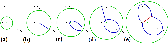
\includegraphics[width=0.95\columnwidth]{figs/sweepcircle/2sites_new.PNG}
\end{center}
%\makebox[0.3in]{}{(a)} \makebox[1.1in]{}{(b)} \makebox[1.0in]
%{}{(c)} \makebox[1.15in]{}{(d)} \makebox[1.35in]{} {(e)}
\vspace{-0.1in}\caption{Illustration of sweep circles for two sites.
The beach curve consists of elliptic segments, each of which
corresponds to a site. The elliptic segment is the bisector of the
corresponding site and the sweep circle. The vertices of the beach
curve trace out the bisector between two sites. The sweep circle,
the beach curve and the bisector are drawn in green, blue and red,
respectively. } \label{fig:sweepcircleprocess}
\end{figure*}

Since two neighboring elliptic segments trace out an active Voronoi
edge and two neighboring active Voronoi edges sandwich an elliptic
segment, we use pointers to maintain the relationship between
ActiveEdge and EllipticSegment. We also use a balanced binary tree
to dynamically maintain the beach curve that contains the elliptic
segments in a circular order. The complete structure of the Voronoi
diagram, such as the incident edges of a Voronoi vertex and the
bounding edges of a Voronoi cell, can be induced from the above data
structures. The pseudo code of our untransformed sweepcircle algorithm is shown
in Algorithm~1.

\begin{algorithm}
\label{alg:pseudocode}
\caption{Untransformed sweepcircle algorithm
for computing 2D Voronoi diagram}
\begin{algorithmic}[1]

\State {\bf Input:} A set of 2D sites $S=\{s_1,\cdots,s_n\}$ and the center of
the sweep circle $c$;
\State {\bf Output:} The Voronoi diagram of $S$
\State  //$\mathcal{T}:$ a binary tree to maintain the beach curve;
\State  //$\mathcal{V}:$ the Voronoi vertex and edge structure;
\State  //$\mathcal{Q}:$ the priority queue of discrete events
\State  Push $n$ touching events into $\mathcal{Q}$ sorted by
$\|c-s_i\|$, $1\leq i\leq n$.
\While {$\mathcal{Q}.isEmpty()==false$}
    \State Pop up the top event $q$ from $\mathcal{Q}$;
    \If {$q$ is a touching event}
        \State Insert a new ellipse $E$ into $\mathcal{T}$;
        \State //Suppose $E$ splits the existing elliptic segment
        \State //$E'$ into $E'_1$ and $E'_2$, and let $p$ be the intersection
        \State //point.
        \State Build two radial edges rooted at $p$, one shared by $E'_1$ and $E$, the other shared by $E$ and $E'_2$;
        \State Compute the time when $E$, $E'_1$, and $E'_2$ disappear;
        \State Push the vanishing event into $\mathcal{Q}$;
    \ElsIf {$q$ is not out of date}
        \State //$q$ is a vanishing event.
        \State //Let $E$ denote the vanishing
        \State //elliptic segment, $E_1$ and $E_2$ the two neighboring
        \State //elliptic segments. If one of them is out of data,
        \State //so is the event. see~Figure~\ref{fig:invalidevents}.
        \State Create a Voronoi vertex $v$;
        \State Terminate the two active edges, joined by $E$, at $v$;
        \State Update the Voronoi structure $\mathcal{V}$;
        \State Create an active Voronoi edge $e$;
        \State Push a vanishing event according to $e$ and its neighboring active edges into the queue $\mathcal{Q}$;
    \EndIf
\EndWhile
\end{algorithmic}
\end{algorithm}

\subsection{Correctness}\label{sec:correctness}

\begin{figure*}[!htbp]
%\vspace{-8mm}
\centering
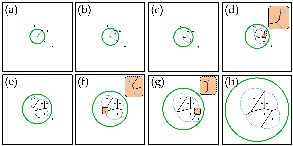
\includegraphics[width=1\linewidth]{figs/sweepcircle/sweepcircleExample3.PNG}
\vspace{-0.1in}\caption{Applying the sweep circle algorithm to a
domain with five sites. (a) The sweep circle touches the first site.
(b) The sweep circle touches the second site. (c) The vertices of
the beach curve, at which two ellipses cross, trace out the bisector
of the two corresponding sites. (d) An elliptic segment (in red) is
vanishing, as a result, the neighboring two segments will eventually
meet. The intersection point is a Voronoi vertex. (e) The circle is
expanding toward the fifth site. (f) The sweep circle touches the
fifth site. (g) The beach curve follows the growing sweep circle and
the vertices of the beach curve trace out the Voronoi edges. (h) The
algorithm stops when the event queue is empty. At this moment, the
Voronoi diagram structure has been fully determined. The beach curve
and the Voronoi edges are drawn in blue and black, respectively. The
vanishing elliptic segments are highlighted in red (see the
insets).} \label{fig:sweepcircleExample}
\end{figure*}

This subsection proves the correctness of our untransformed sweepcircle
algorithm. Consider a set of 2D sites $S=\{s_1,s_2,\cdots,s_n\}$.
Let us denote $\odot(c,R)$ by the sweep circle centered at $c$ with
radius $R$.
 %with radius $R$ such that $c\neq s_i$ for any $1\leq i \leq n$.
  \vspace{0.2in}
\begin{lemma}\label{lema1} Each elliptic segment of the beach curve
bisects the sweep circle $\odot(c,R)$ and the corresponding site
$s_i$. When the center $c$ coincides with a site $s_i$, the elliptic
segment degenerates into a circular arc.  \end{lemma}
\vspace{0.1in}\noindent\textit{Proof:}~~Let $e_i$ be the ellipse
corresponding to site $s_i$, i.e., $e_i=\{x|\|x-c\|+\|x-s_i\|=R\}$.
For any point $x\in e_i$, the shortest distance between $x$ and the
sweep circle is $d\big(x,\odot(c,R)\big)=R-\|x-c\|=\|x-s_i\|$. Thus,
the ellipse is the bisector of the sweep circle and $s_i$. When
$c=s_i$, we obtain $\|x-c\|=\frac{R}{2}$, which is a circle.

\vspace{0.1in}
\begin{lemma}\label{lema2} For any two sites satisfying
$\|c-s_i\|<R$ and $\|c-s_j\|<R$, the ellipses
$$e_i=\{x|\|x-c\|+\|x-s_i\|=R\}$$
and
$$e_j=\{x|\|x-c\|+\|x-s_j\|=R\}$$
intersect at exactly two points, which are on the bisector of $s_i$ and
$s_j$.
\end{lemma}
\vspace{0.1in}\noindent\textit{Proof:}~~The number of intersection
points of two ellipses is from $0$ to $4$. First, the number of
intersection points of $e_i$ and $e_j$ is at least $2$ since:
%\begin{figure}[!h]
%\vspace{-2mm}
%\centering
%\includegraphics[width=1.5in]{figs/envelop3.png}
%\vspace{-0.2in}
%\end{figure}
\vspace{0.1in}
\begin{itemize}
\item The two ellipses share the focus point $c$, which is completely inside the ellipses $e_i$ and $e_j$.
\item Let $p_i\in e_i$ (resp. $p_j\in e_j$) be the closest point on $e_i$ (resp. $e_j$) to the sweep circle $\odot(c,R)$. Then $p_i$ is outside of $e_j$ and $p_j$ is outside of $e_i$ (see the above figure).
\end{itemize}
On the other hand, the intersection points between $e_i$ and $e_j$
satisfy $\|x-s_i\|=\|x-s_j\|$ that determines a straight line $L$. Any intersection point in $e_i\bigcap e_j$
must be a subset of $L\bigcap e_i$ (or $L\bigcap e_j$). This implies that the number of intersections
cannot exceed 2. Therefore, the two ellipses $e_i$ and $e_j$ meet at exactly
two points, which determine the bisector of $s_i$ and $s_j$.

%\noindent\textbf{Remark}~~For the degenerate case
%$\|cs_i\|=\|cs_j\|=R$, the ellipses become line segments of equal
%length, which meet at $c$. Again, $c$ lies on the bisector of $s_i$
%and $s_j$.

\vspace{0.1in}
\begin{lemma}\label{lema3} The beach curve is a closed star
shape with center $c$, and is always inside the sweep circle
$\odot(c,R)$.
\end{lemma}
\vspace{0.1in}\noindent\textit{Proof:}~~Let $e_i$ be the ellipse
corresponding to the site $s_i$, i.e., $\|x-c\|+\|x-x_i\|=R$. Clearly, the
ellipse $e_i$ is inside the sweep circle $\odot(c,R)$, since
$\|x-c\|\leq R$. Let $\Omega=\bigcup_{s_i\in\odot(c,R)} \{x\mid
\|x-c\|+\|x-s_i\|\leq R\}$ denote the union of the ellipses which
are inside the sweep circle. The beach curve is the boundary of
$\Omega$. Due to the fact $\partial\circ\partial=0$, the beach curve
is closed.

%When two non-degenerate ellipses $e_i$ and $e_j$ intersect, by
%Lemma~\ref{lema2}, the two intersection points define the bisector
%of $s_i$ and $s_j$, denoted by $l_{ij}$. The bisector $l_{ij}$
%splits each ellipse into two parts, one containing the corresponding
%site and the other containing the center $c$. As the latter is
%always inside the other ellipse, only the former contributes to the
%beach curve. Observing that all ellipses share a common focus point
%$c$, the beach curve is a star shape with center $c$.
Then we show $\partial \Omega$ is star shaped. Observe that each
ellipse $\|x-s_i\|+\|x-c\|=R$ is a star shape with respect to the
center $c$. Assume the beach curve is not a star shape w.r.t $c$,
there must exist two points $p_i\in e_i,p_j\in e_j$ on the beach
curve such that $p_i,p_j,c$ are collinear and $p_j$ is between $p_i$
and $c$. Therefore, $p_j$ is totally inside $e_i$ since $e_i$ itself
forms a star shape w.r.t. $c$. This contradicts to the assumption
that $p_j\in e_j$ is on the beach curve, which is the boundary of
$\bigcup e_i$.

\vspace{0.1in}
\begin{lemma}\label{lema4_1}
The shortest distance between the center $c$ and the beach curve is
at least $\frac{R-d}{2}$, where $d$ is the distance between $c$ and
the nearest site.
\end{lemma}
\vspace{0.1in}\noindent\textit{Proof:}~~Suppose the $s^{*}$ is the
nearest site to the center $c$. Then the ellipse
$\|x-s^{*}\|+\|x-c\|=R$ must be completely inside the beach curve.
Observe that the shortest distance between the ellipse and the
center $c$ is $\frac{R-d}{2}$. So the shortest distance between the
beach curve and $c$ is at least $\frac{R-d}{2}$.

\vspace{0.1in}
\begin{lemma}\label{lema4}
The elliptic segment corresponding to site $s_i$ is inside the
Voronoi cell of $s_i$.
\end{lemma}
\vspace{0.1in}\noindent\textit{Proof:}~~We distinguish the input
site set $S$ into the \textit{outside} group $S_O=\{s_j|s_j
\notin\odot(c,R)\}$ and the \textit{inside} group
$S_I=\{s_j|s_j\in\odot(c,R)\}$.

We first examine the inside group $S_I$. Let $s_i\in S_I$ be a site
inside the sweep circle and $e_i$ be the corresponding ellipse
$\|x-s_i\|+\|x-c\|=R$. For any point $x\in e_i$, we have
$d(x,s_i)<d(x,s_j)$, $\forall s_j\in S_O$, since the ellipse $e_i$
is the bisector of the sweep circle and the site $s_i$ (by
Lemma~\ref{lema1}).

Then, we prove that $\forall x\in e_i$, $d(x,s_i)\leq d(x,s_j)$ for
any $s_j\in S_I$ by contradiction. Assume there is a point
$\tilde{x}\in e_i$ and a site $s_j\in S_I$ such that
$d(\tilde{x},s_i)> d(\tilde{x},s_j)$. Let $e_j$ be the ellipse of
site $s_j$, i.e., $e_j=\{x|\|x-s_j\|+\|x-c\|=R\}$. Then the point
$\tilde{x}$ must be completely inside the ellipse $e_j$ since
$\|\tilde{x}-s_j\|+\|\tilde{x}-c\|<R$. Observing that the beach
curve is exactly the boundary of the union of ellipses inside the
sweep circle, $\tilde{x}$ is not on the beach curve, which leads to
a contradiction!

Putting it together, the elliptic segment $e_i$ is closer to $s_i$
than any other sites in $S$. Thus, $e_i$ is inside the Voronoi cell
of $s_i$.

\vspace{0.1in}
\begin{lemma}\label{lema5}
The intersection of consecutive elliptic segments of the beach curve
lies on the Voronoi edges.
\end{lemma}
\vspace{0.1in}\noindent\textit{Proof:}~~Suppose $x$ is the
intersection of two consecutive elliptic segments $e_1$ and $e_2$,
corresponding to sites $s_1$ and $s_2$ respectively. By
Lemma~\ref{lema4}, $e_1$ (resp. $e_2$) is inside the Voronoi cells
of $s_1$ (resp. $s_2$). Thus, the intersection of $e_1$ and $e_2$ is
of equal distance to $s_1$ and $s_2$ (and closer to $s_1$ and $s_2$
than any other sites), i.e., it lies on the Voronoi edge.

\vspace{0.1in}
\begin{lemma}\label{lema6}
The Voronoi diagram inside the beach curve has been completely
determined.
\end{lemma}
\vspace{0.1in}\noindent\textit{Proof:}~~For every point $p$ inside
the beach curve, the site which is closest to $p$ can be determined
by the elliptic segment passing through $p$. Thus, the Voronoi
diagram inside the beach curve can be completely determined
regardless of the sites outside of the sweep circle. %\qed

\vspace{0.1in}\begin{lemma}\label{lema7} The current beach curve
contains an elliptic segment corresponding to the site $s_i$ if and
only if $s_i\in\odot(c,R)$ and its Voronoi cell is still open.
\end{lemma}
\vspace{0.1in}\noindent\textit{Proof:}~~ $\Leftarrow$: Assume the
current beach curve still contains one of its elliptic segments, say
$e$. This implies that part of this Voronoi cell lies outside the
current beach curve, which cannot be determined by our algorithm
(see Lemma~\ref{lema6}). Thus, the Voronoi cell is not yet complete,
which contradicts to the assumption that the Voronoi cell of $s_i$
is closed.

$\Rightarrow$: If the Voronoi cell of $s_i$ is still open, it must
intersect the current beach curve at two or more points. Without
loss of generality, consider two intersection points $p_1$ and $p_2$
joined by one or more elliptic segments that are inside the Voronoi cell of $s_i$.
So every point $x$ on this curved segment is closer to
$s_i$ than any other sites, which implies that $x$ satisfies
the equation $\|x-s_i\|+\|x-c\|=R$. Thus, the current beach curve must
contain the elliptic segment of site $s_i$. %\qed

%\begin{figure}[!h]
%\vspace{-4mm}
%\begin{center}
%%\includegraphics[width=0.49\columnwidth]{figs/coverDomain.PNG}
%\includegraphics[width=0.49\columnwidth]{figs/convex.PNG}
%\end{center}
%\vspace{-0.1in}
%\end{figure}
When the algorithm stops, there are exactly $k$ elliptic segments
remaining on the beach curve, corresponding to the $k$ sites on the
convex hull of the input sites $S$, see the above figure.
\begin{figure}[!h]
\begin{center}
\includegraphics[width=0.49\columnwidth]{figs/sweepcircle/coverDomain.PNG}
\includegraphics[width=0.49\columnwidth]{figs/sweepcircle/convex.PNG}
\end{center}
\makebox[0.22\columnwidth]{}{(a)}\makebox[0.46\columnwidth]{}{(b)}
\vspace{-0.1in}\caption{(a) Given the sweep circle $\odot(c,R)$ centered at $c$
with radius $R$, the beach curve is at least $\frac{R-d_0}{2}$ away
from the center $c$ (by Lemma~\ref{lema4_1}), where $d_0$ is the
distance from the nearest site $s$ to the sweep circle center $c$.
By Lemma~\ref{lema6}, the Voronoi diagram inside the beach curve has
been completely determined, so the disk $\odot(c,\frac{R-d_0}{2})$
(the shaded region) provides a rather conservative bound of the
region where the Voronoi diagram has been ready. (b) When the
algorithm terminates, there are exactly $k$ elliptic segments
remaining on the beach curve, corresponding to the $k$ sites on the
convex hull of the input sites $S$.\label{fig:coverDomain}}
\end{figure}


 \vspace{0.1in}\begin{lemma}\label{thm:radiusControl} Let $s$
be the nearest site to the sweep circle center $c$ and $d_0=\|c-s\|$.
Given the sweep circle $\odot(c,R)$, the disk
$\odot(c,\frac{R-d}{2}$


the already-determined Voronoi diagram inside
$\odot(c,\frac{R-d_0}{2})$ has been completely determined.
Especially, when $c$ is exactly one of the sites, the known Voronoi
region is covered by $\odot(c,\frac{R}{2})$. When the algorithm
stops, there are exactly $k$ elliptic segments remaining on the
beach curve, corresponding to the $k$ sites on the convex hull of
the input sites $S$.
\end{lemma}
\vspace{0.1in}\noindent\textit{Proof:}~~According to
Lemma~\ref{lema3}, the ellipse $\|x-s\|+\|x-c\|=R$ must be totally
enclosed inside the beach curve. Also, the perihelion of the ellipse
(with $c$ being the main focus) is closer to $c$ than any other
points on the ellipse.  Therefore, as shown in
Figure~\ref{fig:coverDomain}, the Voronoi diagram inside the disc
$\odot(c,\frac{R-d_0}{2})$ has been completely determined. When $c$
is exactly one of the sites, i.e., $d_0=0$, the Voronoi diagram
inside $\odot(c,\frac{R}{2})$ is completely known.

Furthermore, with sufficiently large radius $R$, all the Voronoi
vertices can be enclosed in the the disc $\odot(c,\frac{R-d_0}{2})$,
which implies that all the Voronoi cells are closed and totally
inside the beach curve except those sites locating on the convex
hull of the site set $S$. By Lemma~\ref{lema7}, there are $k$
elliptic segments remaining on the beach curve, corresponding to the
$k$ sites on the convex hull. %\qed
%
%
%\vspace{0.1in}
%\begin{theorem}\label{thm2}
%All the Voronoi edges are fully determined when the radius of the
%sweep circle $R>2d$, where $d=\max_{1\leq i\leq n}\|cs_i\|$ is the
%distance from the center $c$ to the farthest site.
%\end{theorem}
%\vspace{0.1in}\noindent\textit{Proof:}~~Let $s_i$ is the farthest
%site to the center $c$ and $d\triangleq\|s_i-c\|$. Therefore, when
%the radius $R>d$, all the sites have been touched by the sweep
%circle and are now inside the beach curve. Since the edges of all
%closed Voronoi cells are inside the convex hull of the sites, by
%Lemma~\ref{lema7} these edges are determined.
%\begin{figure}[!h]
%\centering
%\includegraphics[width=0.75\linewidth]{figs/convex.PNG}
%\end{figure}
%Let $C$ is the convex hull of all sites and $k$ be the number of
%sites of $C$. Then the current beach curve ($R>d$) contains exactly
%$k$ elliptic segments, each of which corresponds to an open Voronoi
%cell. The Voronoi edges of these cells can be determined by tracing
%out the vertices of neighboring elliptic segments, see the above
%figure. \qed

\begin{figure}
\vspace{-2mm}
\begin{center}
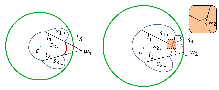
\includegraphics[width=0.9\columnwidth]{figs/sweepcircle/invalidEvt.png}
\end{center}
%\makebox[0.18\columnwidth]{}{(a)}\makebox[0.39\columnwidth]{}{(b)}
\vspace{-0.1in}\caption{Out of date events. The red elliptic segment
is sandwiched by two Voronoi edges, say $l_1$ and $l_2$, and will
vanish when the sweep circle touches the point $w_1$. As a result, a
vanishing event $q$ has been pushed into the priority queue
$\mathcal{Q}$. However, when the sweep circle touches the site
$s_4$, the edge $l_1$ is intercepted by a newly-created Voronoi edge
(see the inset). Therefore, the event $q$ is out of date when it is
popped from the queue $\mathcal{Q}$, which is simply ignored by the
sweep circle algorithm.} \label{fig:invalidevents}
\end{figure}

%\noindent\textbf{Remark}~~In our sweep circle algorithm, the circle
%center can be an arbitrary point. Let $d=\max_{1\leq i \leq n}
%\|cs_i\|$ be the maximal distance from the center to the site. By
%Theorem~\ref{thm2}, the algorithm terminates when the radius $R>2d$.
%In practice, we can set $c$ the centroid of $S$, which can reduce
%the terminating radius. Furthermore, our algorithm also works for
%the case that the center $c$ coincides with a site.


Finally, the following theorem reveals the relationship between the
sweep line algorithm and our untransformed sweepcircle algorithm.
\vspace{0.1in}
\begin{theorem}\label{thm1}
The Fortune's sweep line
algorithm~\cite{Fortune1986} is a degenerate form of our sweepcircle algorithm if the center $c$ is at infinite distance to the
sites.
\end{theorem}
\vspace{0.1in}\noindent\textit{Proof:}~~The site $s_i$ contributes
to the beach curve \textit{after} the sweep circle hits $s_i$ and
\textit{before} the corresponding Voronoi cell becomes a closed
polygon. During this period, the elliptic segment of $s_i$ is inside
this Voronoi cell (by Lemma~\ref{lema4}) and it is closer to the
focus point $s_i$ than the other focus point $c$, the center of the
sweep circle since $c$ is assumed to be at infinite distance to the
sites. The distance between $s_i$ and its elliptic segment is very limited, and cannot exceed the size of $s_i$'s Voronoi cell.

Under this condition, if the center $c$ is at infinite distance to $s_i$, the eccentricity
of the ellipse approaches $1$. As a result, the sweep circle becomes
a straight line and the elliptic segment becomes a parabola segment.
At the same time, the beach curve still serves as the bisector of the sweep line and
the active sites, exactly the same situation with that achieved in Fortune's sweep line algorithm. Therefore, we can conclude that Fortune's sweep line algorithm is the
degenerate form of our untransformed sweepcircle algorithm. %\qed


\subsection{sweepcircle-Complexity}
\label{subsec:sweepcircle-complexity}

\begin{theorem}\label{thm3}
The untransformed sweepcircle algorithm computes the Voronoi diagram in $O(n\log
n)$ time and requires $O(n)$ space.
\end{theorem}

\vspace{0.1in}\noindent\textit{Proof:}~~First of all, sorting the sites according to
the distances to the sweep center requires $O(n\log n)$ time. In the following, we come to analyze the time cost of the sweeping process.

First, we show the number of
elliptic segments, as well as that of the events, is $O(n)$. There
are two kinds of events, namely, the touching event and the
vanishing event. The number of touching events is equal to the
number of sites $n$. When the sweep circle touches a new site, the
algorithm splits an existing elliptic segment of the current beach
curve into two and then add a new elliptic segment corresponding to
the new site. Therefore, at most $2n$ elliptic segments are
generated, and at most $3n$ vanishing events need to be considered
throughout the algorithm. Note that some vanishing events may be
out of date and are discarded when the sweep circle progresses (see
Figure~\ref{fig:invalidevents}).

Second, we show handling each event takes $O(\log n)$ time. For the
touching event, a new elliptic segment is inserted into the beach
curve, maintained by a balanced binary tree $\mathcal T$. The
insertion takes $O(\log n)$ time. For the vanishing event, the
priority queue $\mathcal Q$ is updated, which also takes $O(\log n)$
time.

Third, the Voronoi diagram, the balanced binary tree and the priority queue require
$O(n)$ space to store the vertex-edge structure, the $O(n)$ elliptic segments and $O(n)$
events respectively.

Putting it altogether, the sweep circle algorithm takes $O(n\log
n)$ time and requires $O(n)$ space. %\qed

\vspace{-0.1in}
\section{Parallel Sweep Circles}\label{sec:sweepcircle-parallel}
\vspace{-0.1in} To compute the Voronoi diagram in a parallel
fashion, we need to partition the domain and then solve each
sub-domain independently. To use the sweep line algorithm, one needs
to place the initial sweep line at one side of the to-be-computed
region, and then moves it in a certain direction across such region.
As shown in Figure~\ref{fig:sweeplineDrawback}, the sweep line
algorithm needs to sweep the region much larger than the desired
region. Furthermore, as only the centered region is correct, one has
to trim the computed Voronoi diagram to get the final result.

Compared to the classical sweep line algorithm, the proposed untransformed sweepcircle algorithm has two unique advantages, which makes it
preferable for parallel implementation. First, the sweep circle can
be placed anywhere in the domain. Second, the beach curve of our
sweepcircle algorithm is closed and the Voronoi diagram inside the
beach curve can be completely determined regardless of the sites
outside the sweep circle. Thus, each sweep circle thread can work
independently. Even though the sweep circles may have overlap, we
do not need any postprocessing to trim the Voronoi diagram.

Given a 2D domain $\Omega$ containing sites $S$, we can partition
the domain $\Omega$ into disjoint sub-regions, $\Omega=
\bigcup_{i=1}^{m}\Omega_i$, $\Omega_i\bigcap\Omega_j=\emptyset$,
$\forall i\neq j$. Then each sub-region $\Omega_i$ is assigned a
sweep circle thread, which places a sweep circle at arbitrary
location inside $\Omega_i$. In practice, one can set the center
$c_i$ the barycenter of $\Omega_i$. Each thread stops when its event
queue is empty. If one sub-region contains no sites at all, we can
merge that region with neighboring region such that each sub-region
contains at least one site. The pseudo code of the parallel sweep
circle algorithm is shown in Algorithm 2.
\begin{algorithm}[!h]
\label{alg:pseudocode2}  \caption{Parallel sweep circle algorithm}
\begin{algorithmic}
\State {\bf Input:} A 2D region $\Omega$ containing $n$ sites
$S=\{s_1,\cdots,s_n\}$ and a partition of $\Omega$ into $m$ disjoint
sub-regions $\Omega_{i}$, $\Omega_{i}\bigcap \Omega_{j}=\emptyset$
$\forall i\neq j$.

\State {\bf Output:} The Voronoi diagram of $S$

\State \textcolor{blue}{\textbf{parallel}} \textbf{for} each
sub-region $\Omega_i$ \textbf{do}

\State ~~~ Compute the barycenter $c_i$ of $\Omega_i$

\State ~~~ Run the sweep circle algorithm centered at $c_i$

\State \textcolor{blue}{\textbf{parallel}} \textbf{end for}
\end{algorithmic}
\end{algorithm}



In fact, since each sweep circle thread cares for only the Voronoi
structure inside $\Omega_i$, we can modify the sweep circle
algorithm such that it can terminate early, i.e., without processing
all the vanishing events in the event queue.  By Lemma~\ref{lema6},
the Voronoi diagram inside the beach curve is complete. Thus, we can
test whether the beach curve contains the entire sub-region
$\Omega_i$. If so, we can stop the sweep circle algorithm for
$\Omega_i$. In practical application, the sub-region $\Omega_i$ is
usually modeled by a polygon. So this test can be implemented
easily. Let $R_s$ denote the radius of the sweep circle when the
algorithm stops. The following theorem provides an upper bound of the
stopping radius $R_s$:

\vspace{0.1in}\begin{theorem}\label{thm_r} Given the sub-region
$\Omega_i$, let $\odot(c_i,r_i)\supset\Omega_i$ be the smallest
covering disc. The site $s\in\Omega_i$ is the nearest one to the
center $c_i$. Define $d=\|c_is\|$. The sweep circle algorithm for
the sub-region $\Omega_i$ can stop when the radius $R_s\geq 2r_i+d$
or the event queue is empty, or whichever occurs first.\end{theorem}
%\begin{figure}[!h]
%\begin{center}
%\includegraphics[width=0.49\columnwidth]{figs/coverDomain.PNG}
%\end{center}
%\vspace{-0.1in}\caption{Given the sweep circle $\odot(c,R)$ centered at $c$ with
%radius $R$, the beach curve is at least $\frac{R-d_0}{2}$ away from
%the center $c$ (by Lemma~\ref{lema4_1}), where $d_0$ is the distance
%from the nearest site $s$ to the sweep circle center $c$. By
%Lemma~\ref{lema6}, the Voronoi diagram inside the beach curve has
%been completely determined, so the disk $\odot(c,\frac{R-d_0}{2})$
%(the shaded region) provides a rather conservative bound of the
%region where the Voronoi diagram has been
%ready.\label{fig:coverDomain}}
%\end{figure}
\vspace{0.1in}\noindent\textit{Proof:}~~By Lemma~\ref{lema3}, the
ellipse $\|x-s\|+\|x-c_i\|=R$ must be inside the beach curve, since
$s$ is the nearest site to the center $c_i$. By Lemma~\ref{lema4_1},
the beach curve can contain a disc $\odot(c_i,\frac{R-d}{2})$
completely. In order to ensure that the Voronoi diagram inside
$\Omega_i$ has been fully determined, we require the terminating
radius $R_s$ satisfying $\frac{R_s-d}{2}\geq r_i$, which completes
the proof. %\qed
\begin{figure}[!htbp]
\vspace{-2mm}
\begin{center}
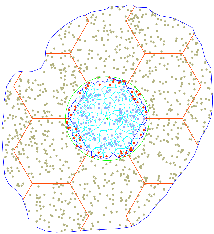
\includegraphics[width=0.9\columnwidth]{figs/sweepcircle/overlap.png}\\
\end{center}
\vspace{-0.1in}\caption{In practice, the beach curve follows the
sweep circle very closely, which leads to a small stopping radius
$R_s$. For a domain $\Omega$ with 1000 randomly distributed sites,
we partition $\Omega$ into equally sized regular hexagons and
compute the ratio of the number of sites inside the hexagon to the
number of sites inside the sweep circle. The average ratio of 10
experiments is $71.9\%$, which implies that the parallel sweep
circle algorithm is very effective, since only less than $28.1\%$
computation is ``wasted''.} \label{fig:overlap}
\vspace{-2mm}
\end{figure}

We would like to point out the above upper bound of the stopping
radius $R_s=2r_i+d$ is very conservative. Based on our experiments,
we observe that the beach curve usually follows the sweep circle
very closely. As a result, the stopping radius is usually slight
larger than the size of the sub-region $r_i$. In practice, we can
partition the domain into equally sized regular hexagon, which is
very effective to reduce $R_s$. The theoretical lower bound of $R_s$
is $R_s=r_i$, which occurs for the uniformly distributed sites with
such hexagonal partition.

Furthermore, as the Voronoi diagram inside the beach curve is
guaranteed to be correct, the overlap among the sweep circles does
not affect the final result. This feature significantly
distinguishes our algorithm from the sweep line algorithm, which has
to trim the computed voronoi diagrams.


\vspace{-0.1in}
\section{Experimental Results}\label{sec:sweepcircle-results}
\vspace{-0.1in} We implemented our untransformed sweepcircle
algorithm in C++ and tested it on a PC with an Intel Xeon 2.50GHz
CPU and 8GB memory. The graphics card is an NIVDIA GTX 580 with 512
cores and 1.5GB memory. Our program is compiled using CUDA4.0 RC2.

We have shown that the sweep circle has the same time and space
complexity as the sweep line algorithm. To measure and compare the
practical performance, we count the number of discrete events for
the sweep circle algorithm and the sweep line algorithm. We randomly
generate up to 1000 sites in a unit square and then run the
sequential sweep circle and sweep line algorithms. Although based on
different sweeping strategies, both approaches have very similar
number of events, as shown in Figure~\ref{fig:events}. Due to the
trigonometric functions used for computing the joint point between consecutive elliptic segments, its
computational cost for processing each event is slightly higher than
that of the sweep line algorithm. As a result, the single-core sweep
circle algorithm is slower than the sweep line algorithm. However,
as mentioned before, the proposed sweep circle algorithm is superior
than the sweep line algorithm due to its parallel nature. With the
parallel untransformed sweepcircle algorithm, the average number of events can be
significantly reduced by increasing the number of sweep circles.

\begin{figure}[!htbp]
\vspace{-3mm}
\begin{center}
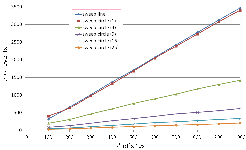
\includegraphics[width=0.95\columnwidth]{figs/sweepcircle/num_of_events.png}\\
\end{center}
\vspace{-0.1in}\caption{Both the sequential sweep circle and sweep
line algorithms have very similar number of discrete events. With
the parallel sweep circle algorithm, the average number of events
for each GPU thread is significantly reduced. The horizontal axis
and the vertical axis show the number of sites and the average
number of discrete events respectively. The number in the bracket
represents the number of sweep circles.} \label{fig:events}
\vspace{-3mm}
\end{figure}


Figure~\ref{fig:gpuSweepcircle} shows an example of 250 sites within
an irregular domain, which is partitioned into $m^2$ ($m=2,3,4,5$)
sub-regions. Each sub-region $\Omega_i$ is assigned a GPU based
sweep circle thread, which outputs the Voronoi diagram inside the
corresponding beach curve. Although the neighboring beach curves
have overlap when the sweep circles progress, all the threads can
run independently without any data conflicts or synchronization.
\iftrue
\begin{figure}[!htbp]
\vspace{-3mm}
\begin{center}
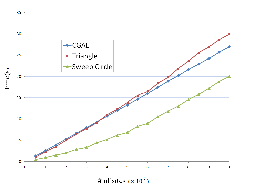
\includegraphics[width=0.9\columnwidth]{figs/sweepcircle/timeCompare.png}\\
\end{center}
\vspace{-0.1in}\caption{The comparisons with CGAL~\cite{cgal} and
Triangle~\cite{Shewchuk:1996} show that our sweep circle algorithm has
parallel speedup ratio of $1.63$ and $1.73$ respectively. The
horizontal axis and the vertical axis shows the number of sites
and computing time respectively.} \label{fig:Comparison}
\vspace{-3mm}
\end{figure}
\fi
Figure~\ref{fig:Comparison} demonstrates a comparison of our sweep circle
algorithm with CGAL~\cite{cgal} and Triangle~\cite{DBLP:conf/wacg/Shewchuk96}. In
this experiment, the number of sweep circles of our algorithm is $25$.
Due to the limitation of time, our implementation has not been optimized.
But our sweep circle algorithm still shows satisfactory parallel speedup
ratio. Considering that modern Graphics Computing Devices always have
hundreds of cores, our algorithm has great potential of speedup.

\begin{figure*}[!htbp]
\vspace{-6mm}
\centering
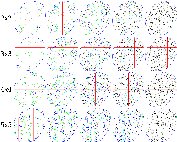
\includegraphics[width=0.85\linewidth]{figs/sweepcircle/gpuSweepcircle.PNG}
\vspace{-0.1in}\caption{Parallel computing Voronoi diagram using GPU
based sweep circle algorithm. The entire domain is uniformly divided
into $m^2$ sub-regions (where $m=2,3,4,5$ for this experiment), and
a sweep circle thread is run for each sub-region independently. The
intermediate results are shown in the left and the right most column
is the final result. The active edges, the sweep circle and the
beach curve are drawn in cyan, green and blue, respectively.}
\label{fig:gpuSweepcircle}
\end{figure*}

Our algorithm can be applied to 3D surface by using
parameterization. Figure~\ref{fig:3d} shows two genus-0 3D models
which are conformally parameterized to disc and square using the
harmonic map~\cite{DBLP:journals/tmi/GuWCTY04} and the holomorphic
1-form method~\cite{DBLP:conf/sgp/GuY03}. We generate 200 and 600
random sites on the 3D face and sheep model. Then we run the
parallel sweep circle algorithm on the 2D parametric domain using
the Euclidean distance and the parameterization induces the Voronoi
diagram on the 3D surface. See Figure~\ref{fig:3dresults}. An
interesting work is to use the geodesic distances instead of the
Euclidean distance, which would result in an intrinsic geodesic
Voronoi diagram on surface. As this is beyond the scope of this
report, we will address it in the future work.

%We conducted experiments on a computer with a configuration of ??,
%where about $100$ GPU threads are available. Although the computing
%power of each GPU thread is only about one twentieth of CPU's
%computing capability, the GPU based sweep circle algorithm still
%runs twice faster than the optimized implementation of the CPU based
%sweep line algorithm. The detailed comparison is illustrated in
%Figure~\ref{fig:performanceComparedWithSweepline}.
% \begin{figure}[!htbp]
%\centering
%\includegraphics[width=\columnwidth]{figs/performanceComparedWithSweepline.PNG}
% \vspace{-0.1in}\caption{} \label{fig:performanceComparedWithSweepline}
%\end{figure}

%%===================================
The proposed sweep circle framework can be easily extended to the
additively weighted Voronoi diagram, for which the conventional
Euclidean distance is modified by the weights assigned to each site. We
represent each site $s_i$ as a disk of radius $r_i$ centered at
$s_i$, where $r_i$ is the weight of site $s_i$. The active edge
structure is also modified to contain both the line segments and
hyperbolic segments, as shown in Figure~\ref{fig:averageUV}.


\begin{figure}[!htbp]
\begin{center}
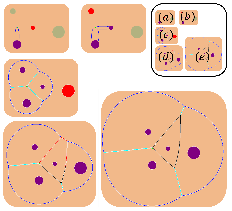
\includegraphics[width=0.9\columnwidth]{figs/sweepcircle/weightedVoronoi.png}
\end{center}
\vspace{-0.1in}\caption{Computing the additively weighted Voronoi
diagram, where the conventional Euclidean distance is modified by the
weights assigned to the generator sites. The weights are illustrated
by the size of the site. The resulting Voronoi diagram contains both
hyperbolic segments and line segments. The animation from (a) to (e)
illustrates the sweeping process. } \label{fig:averageUV}
\vspace{-2mm}
\end{figure}


\begin{figure}
\begin{center}
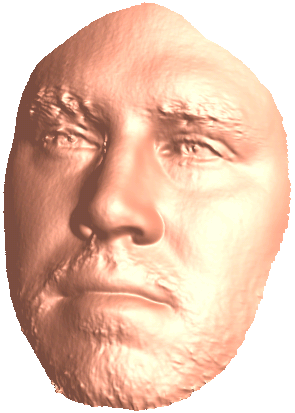
\includegraphics[height=1.75in]{figs/sweepcircle/dale_3d.png}
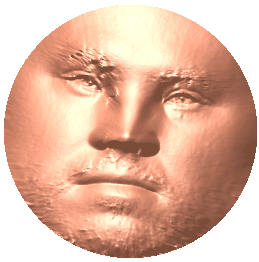
\includegraphics[height=1.75in]{figs/sweepcircle/dale_uv.png}\\
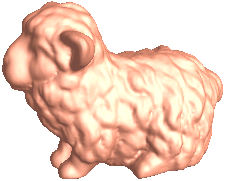
\includegraphics[width=1.45in]{figs/sweepcircle/sheep_3d.png}
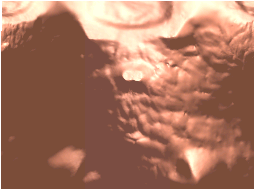
\includegraphics[width=1.55in]{figs/sweepcircle/sheep_uv.png}\\
\end{center}
\caption{3D models and their parameterization.} \label{fig:3d}
\end{figure}

\begin{figure*}[!htbp]
\begin{center}
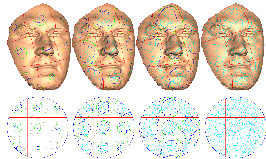
\includegraphics[width=0.925\linewidth]{figs/sweepcircle/dale.png}\\
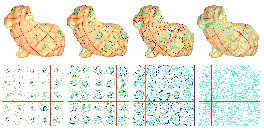
\includegraphics[width=0.925\linewidth]{figs/sweepcircle/sheep.png}\\
\end{center}
\caption{Our method can be applied to 3D surfaces by using
parameterization.} \label{fig:3dresults}
\end{figure*}


%%===================================

\vspace{-0.1in}
\section{Discussion}\label{sec:sweepcircle-discussion}
\vspace{-0.1in}
Generally speaking, a divide-and-conquer Voronoi algorithm needs to overcome
two difficulties: 1)~computing the Voronoi diagram in a sub-domain; and 2)~merging
the separate results into a complete diagram. Taking Figure~\ref{fig:sweeplineDrawback}
for an example, a parallelized sweepline algorithm needs to distinguish the diagram
in the green square from other part for merging purpose, because the computed result
outside the green square may be incorrect. However, our algorithm are different
than the sweepline algorithm to this point, due to the property that our algorithm
guarantees the computed Voronoi diagram behind the beach curve is globally correct.

The robustness is very important for computing Voronoi diagram and Delaunay
triangulation. For example, {\em In-Circle} test is a frequent routine in computing
Delaunay triangulation. The operation, however, is error-prone. Different than the
In-Circle operation, we use a sweepcircle to determine the priority in handling sites.
Suppose $s_1$ and $s_2$ are in a nearly equal distance to the sweepcircle center.
Even if the handling orders of $s_1$ and $s_2$ are reversed due to numerical problems,
it will not affect the final Voronoi diagram since $s_1$ and $s_2$ lead to changes in
different parts of the beach curve. Instead, we found two cases are critical to the
robustness of the sweepcircle algorithm: 1)~When we insert a new elliptic arc
segment $e$, it intersects an existing elliptic arc $e_i$ that nearly vanishes;
and 2) two consecutive elliptic arc segments vanish in a very short time gap.
These cases happen when more than 3 Voronoi cells share a common vertex. In our
implementation, we use a tolerance $1e-7$ to identify if the vanishing point is
a high-order Voronoi vertex.

Thurston~\cite{Thurston:1986} observed the sweepcircle technique allows to compute the Voronoi diagram locally, which shows the Voronoi diagram can be parallelized in nature.
Dehne and Klein~\cite{Dehne_Klein:1987} applied the sweepcircle to compute a type of transformed Voronoi diagram. Although their algorithm also supports multiple sweep circles, it is fundamentally different with our untransformed sweepcircle algorithm.
\begin{enumerate}
\item In the traditional sweepcircle algorithm, the transformed edges are very complicated in representation form. By contrast, our algorithm is easy to implement since the most complicated operation is nothing but an arc-cosine calculation.
\item The beach curve consists of elliptic segments in our untransformed sweepcircle algorithm, while the beach curve is rather complicated in Dehne and Klein's sweepcircle algorithm (they didn't mention the representation form of the beach curve in~\cite{Dehne_Klein:1987}).
\item Our algorithm is very natural to extend onto 2D weighted Voronoi diagrams, while it is not clear whether it is easy or not for Dehne and Klein's sweepcircle algorithm to support 2D weighted Voronoi diagrams.
\item Dehne and Klein's sweepcircle algorithm can be easily extended to the Voronoi diagram on the surface of a cone, while it seems not easy for our algorithm.
\end{enumerate}
\vspace{-0.1in}
\section{Summary}\label{sec:sweepcircle-summary}
\vspace{-0.1in} This chapter presents the untransformed sweepcircle
algorithm for 2D Voronoi diagram. Our algorithm has the optimal
$O(n\log n)$ time complexity and $O(n)$ space complexity. The
classical sweep line algorithm is the degenerate form of our algorithm when the circle center is at infinity. Our
algorithm is flexible in that it allows multiple circles at
arbitrary locations to sweep the domain simultaneously, which
naturally leads to a parallel implementation. It is easy to
implement, without complicated numerical calculation. We demonstrate
the efficacy of our parallel sweep circle algorithm using GPU.
